\documentclass[11pt,english]{article}
\usepackage[T1]{fontenc}
\usepackage[latin9]{inputenc}
\usepackage{geometry}
\geometry{verbose,tmargin=1.5cm,bmargin=1.5cm,lmargin=1cm,rmargin=1cm}
\usepackage{graphicx}
\usepackage{babel}
\begin{document}

\section{
	Analysis of plots
}
\subsection{
Analysis of plot01 ( Average (StepTime and LoopTime over reruns) vs number of iterations) }
\includegraphics[width=7cm]{doc/g05_plot01.eps}
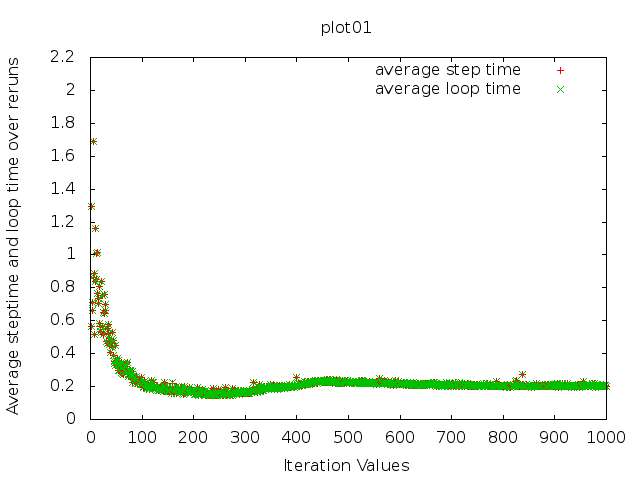
\includegraphics[width=7cm]{doc/g05_plot011.eps}
There are two major observations :-
\begin{enumerate}
\item The stepTime and looptime are very close to each other. This is meaningful because the only major process that is happening inside the loop is Step function and apart from the step function, only a few addition, subtraction and reading is happening.
\item Another interesting thing is that the avg stepTime decreases till iteration value of 100 and then approximately remains constant. Most likely the cause behind this is the behavior of the world of Box2D. Possibly during the initial iterations, many collisions are taking place, which increases the step time in the initial iterations(when the dominoes fall). And then during the later iterations fewer collisions are taking place due to which the step time is less, which drags the average step time down along with it. It is also interesting to observe the graph for upto iteration value 1000, which shows a falling trend, increases slightly and then becomes constant. All this seems to be because of the collisions in the actual world in which the collisions are running.
\end{enumerate}



\subsection{
Analysis of plot02 ( Average (StepTime, CollisionTime, Velocity Time, Position update time over reruns) vs number of iterations) }
\includegraphics[width=8cm]{doc/g05_plot02.eps}
\begin{enumerate}
\item In this case, an important thing to notice is that the collision time, velocity time and position update time add upto the step time. This proves that major things which happens inside the step function are collision handling, velocity update handling and position update handling.
\item The ratio of the time taken by collision handling, velocity update handling, and position update handling is approximately same for different values of iteration number. Which is to say that, if more collisions are happening, then there is a greater need to update velocities and positions, which makes sense

\end{enumerate}


\subsection{
Analysis of plot03 ( Average of step time and looptime over iteration values vs rerun number) }
\includegraphics[width=7cm]{doc/g05_plot03.eps}
\begin{enumerate}
\item The averages of looptime and steptime are same because of reasons mentioned earlier.
\item The avg looptime over iteration values changes slightly for different rerun index. The important thing to notice that it is not constant. And the most likely reason for this is the other processes that runs in CPU during the execution of this program. So say when the nth iteration is running, the load on CPU might increase because of which the avg of step time over iteration values might increase for that particular rerun number. This justifies rerunning the program many times.
\end{enumerate}

\subsection{
Analysis of plot04 (Average of (step time, collision time, position update time, velocity update time over iteration values) vs the rerun number) }
\includegraphics[width=7cm]{doc/g05_plot04.eps}
The analysis is very similar to the previous case. Again here the point that the sum of position update time, velocity update time, and collision update time is almost equal to step time and that the ratios are similar.


\subsection{
Analysis of plot05 (Average of iteration values over reruns (with error bars) vs the iteration values) }
\includegraphics[width=7cm]{doc/g05_plot05.eps}
\begin{enumerate}
\item The new feature is the error bars over plot01. The error decreases as the iteration values increases. On closely observing the step times from the actual data files, many a times the step times initially are very high and many times they are pretty low. This is perhaps because of the way in which the OS allocates CPU to the program. If the CPU is busy then the program gets less CPU initially and it increases into the program. However if the CPU is free then the program quickly gets sufficient CPU power. However when we consider higher iteration values, then the initial disturbance gets averaged out due to which the error is not so visible. 
\end{enumerate}



\subsection{
Analysis of plot06 (frequency of a particular step time vs the step time for iteration value 29) }
\includegraphics[width=7cm]{doc/g05_plot06.eps}
The step time for different reruns are almost in a close range of 0.045ms to 0.050 ms. Approximately 70\% of values are in this range. However in some exceptional cases, the step time came out to be upto 0.1 ms where the CPU load might have increased.


\section{
	Analysis of plots when system is heavily loaded}
\subsection{
	Heavy CPU usage and light memory usage}
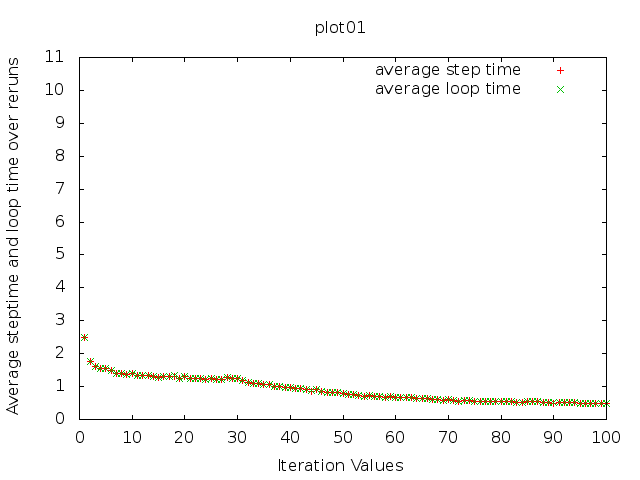
\includegraphics[width=7cm]{doc/g05_plot01_cpu.eps}
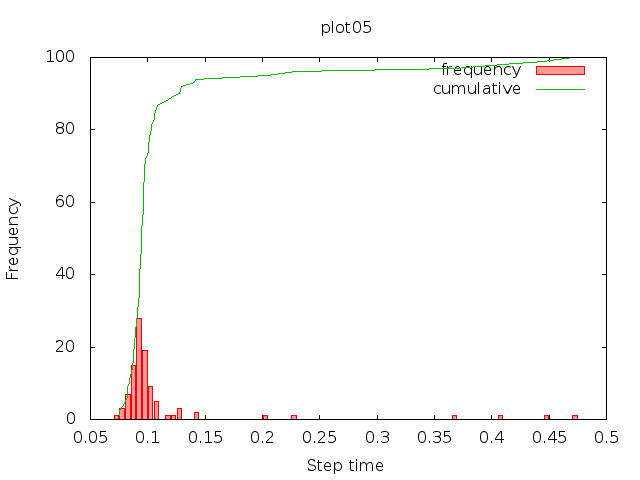
\includegraphics[width=7cm]{doc/g05_plot06_cpu.eps}
I increased the CPU load by running 3 computationally heavy processes which don't comsume a lot of memory (a simple infinite while loop which does a lot of computation inside the while loop). The effect was predictable. The average step time went up by about 2.5 timesas shown in the first graph. Another very interesting observation here is that in the frequency of step time in the case of light usage, the maximum of frequency occured at the mimimum value of step time, which meant that there were rare occasions when the step time increased because of other processes. However when the load was heavy, there were rare occasions, when the step time was less and most of the times the step time was much more than the normal time taken. 
\subsection{
	Normal CPU usage and heavy memory usage}
All the graphs are almost identical. This proves that Box2D is not very heavy on memory(atleast the non-graphic version which we ran for this experiment), and doesn't get affected by memory.

\section{
	Changes in the patch of b2Timer.cpp functions}
The change done in the patch was very minor. In the original file, the original time was taken in ms in integers and the final time was considered in ms in integers and then subtracted. So as far as $\mu$s is concerned, it was multiplied by 0.001 and then subtracted. So take for instance if the $\mu$s value initially was 89900 and finally it was 90100, then when it was converted to ms then the initial value would have been 89 seconds and final would have been 90 seconds, thus giving a difference of 1 second. However the true difference is 200ms here. So all the patch did was save the $\mu$s in its original value initially and then subtract it from the $\mu$s value finally and then converted to ms and returning it in floating point precision, thus eliminating the error.
\section{
	Difference in using time and gettimeofday function}
For an iteration value of 100000, the real time obtained by using time command is very slightly greater than the total loop time obtained by using gettimeoftheday function. (0.045\% greater). This is most likely because of the initialization of the b2World and other things which are not counted in gettimeoftheday calculations as done in out program.
\\*
Another important feature of time function which is not present with gettimeoftheday function is that time also reports the user time, which basically is the time which the program actually used, discounting the time when the program was blocked, or when other processes were running.


\section{
Profiling Report }

\subsection{Introduction}

We used gprof for profiling our data.

We've generated profiles for 100, 10 thousand,100 thousand and
one million iterations in each of debug mode and release mode(using
both -O2 and -O3 flags )

We've noticed that 
\begin{itemize}
\item for lower iteration values, the profiles were quite random which is
understandable because the actual execution time for small iteration
values is comparable to the sampling time.
\item for large iteration values for example, 100000 and above, the profiles
were quite consistent and almost constant (as the execution time is large
compared to sampling)
\end{itemize}

\subsection{Comparing Profiles}

For iteration value 10L, the beginning parts of the profiles for release
and debug modes are respectively:-

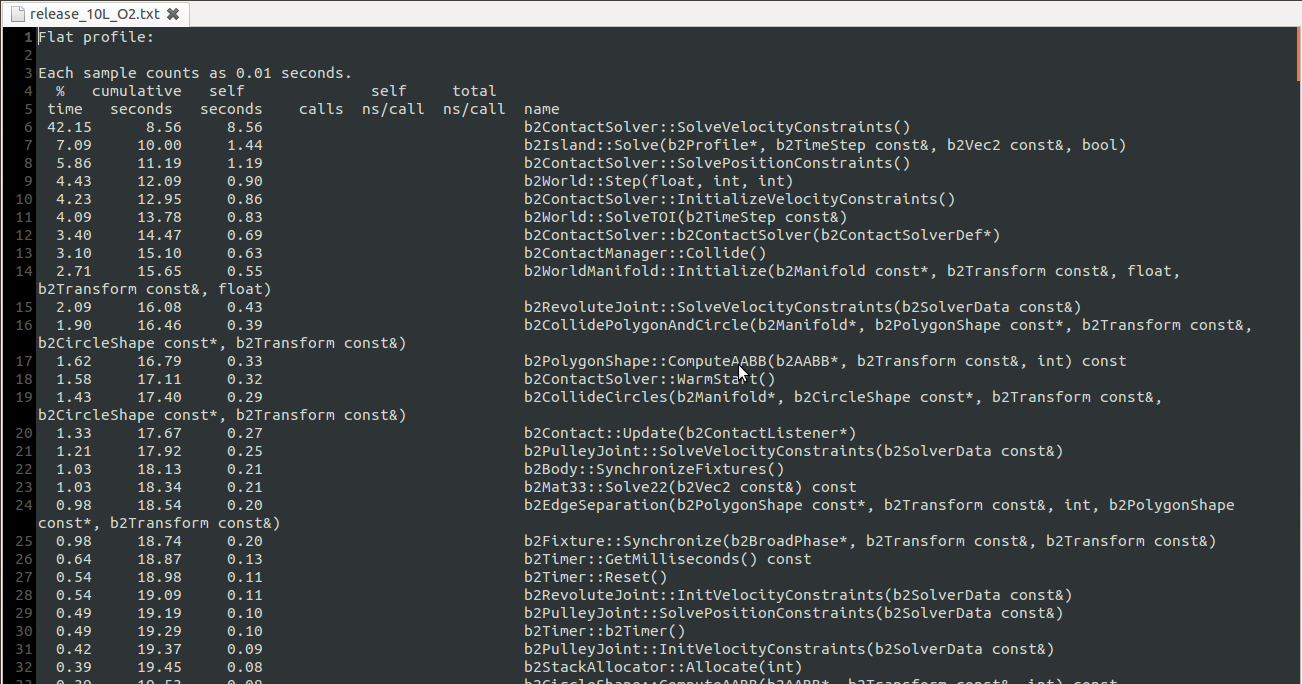
\includegraphics[width=11cm,height=6cm]{doc/croprelease10L.eps}

.

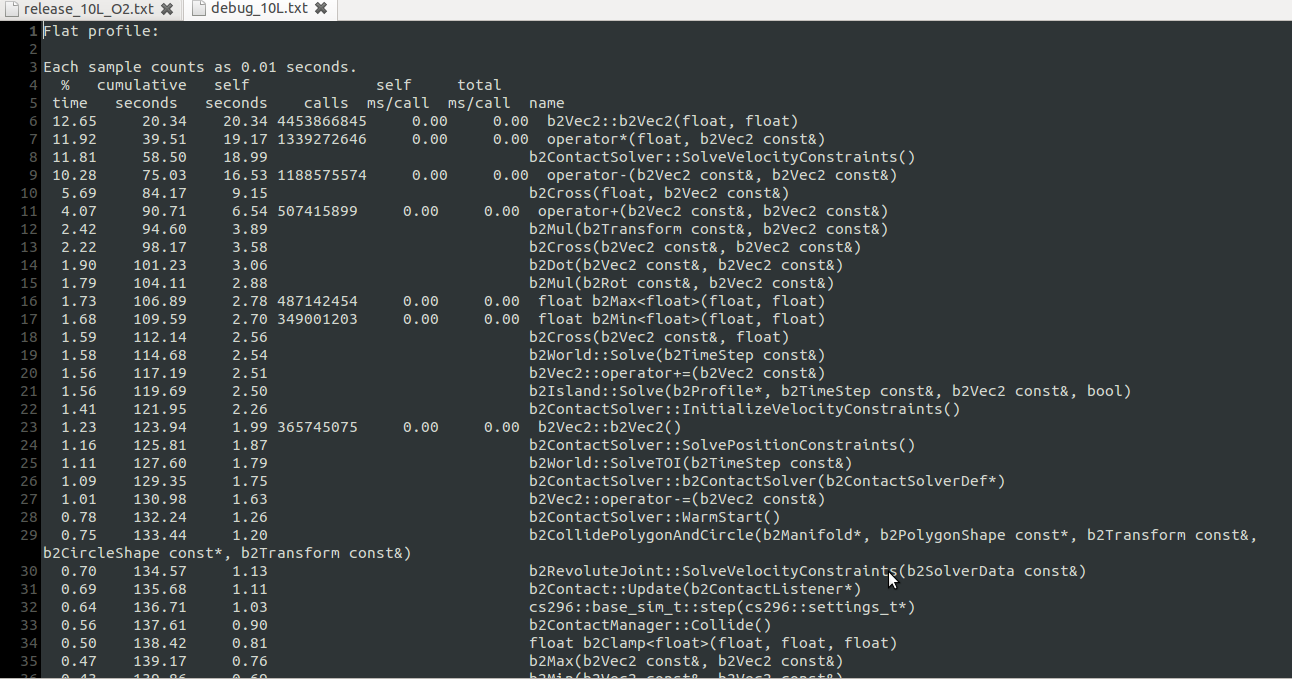
\includegraphics[width=11cm,height=6cm,keepaspectratio]{doc/cropdebug_10L.eps}

\begin{itemize}
\item Not all the functions which were reported in profiling for debug mode
were there in profile for release mode.The reason being many functions
were made inline by the compiler with the use of optimisation flags. (the -O2 flag turns on the -finline-small-functions flag which makes
the small functions inline for better efficiency. also the -O3 flag
turns on the -finline-functions which integrates all simple functions
into their callers)


\item We also see that the executable generated using debug is larger than
that produced by the release version, because compiling in debug mode
also generates some extra data which aids in debugging.

\item We've noticed that for larger iteration values (above 1K) the execution
time for that of debug version is almost 10 times compared to that
of release version. so, these -On flags actually optimize atleast
10 times . This shows that there is actually very high scope for improvement
in the way we write our code.
\end{itemize}

\subsection{Improvements}
\begin{itemize}
\item For our part of the code, the functions operators+,operator-,operator{*}
are called a large number of times by various functions, and the study
of profiles shows that making them inline reduces the time significantly.
These are relatively small functions, and the function call is expensive relative
to their inline form. Since these are small functions, we can directly write
them inline.
\item For the box2d code, definitely the function ``b2ContactSolver::SolveVelocityConstraints()''
can be improved a lot as seen from the study of the two profiles.
It calls many small functions a large number of times, so making all
of them inline can significantly improve the efficiency.
\end{itemize}

\subsection{Call Graphs}

The callgraphs for debug and release mode respectively :

.

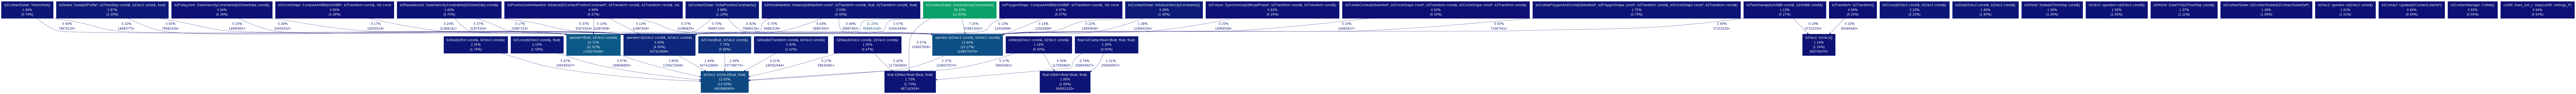
\includegraphics[width=18cm,height=3cm]{doc/debug_10L.eps}

.

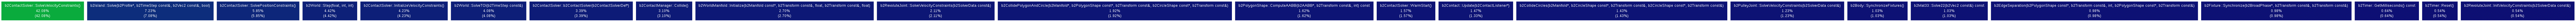
\includegraphics[width=18cm,height=1cm]{doc/release_10L_O2.eps}

The call graphs represent the callee-caller relations. It shows all the functions that called a particular function 
and also all the functions that are called by it.

For release mode, we can see that there are no arcs coming out of
any functions which implies that all the callee functions are made
inline to the caller functions , where as there are a large number
of function calls which are present in callgraphs for debug mode.
\end{document}
